Como enunciamos en la explicaci\'on de nuestro algoritmo, el mismo va chequeando en cada paso si existe alg\'un gimnasio capaz de ser vencido y si existe buscar cual es el m\'as cercano de estos a ser vencidos, por lo tanto existir\'an casos en los cuales la soluci\'on obtenida para los mismos sea la \'optima pero para algunos no lo ser\'a.

Con respecto a las soluciones obtenidas y las \'optimas dado nuestro algoritmo mostraremos las familias de casos en las cuales la soluci\'on obtenida para el greedy es la \'optima:

\begin{enumerate}
\item No se obtiene soluci\'on por no haber las pokeparadas necesarias para ganar en todos los gimnasios.
\item No se obtiene soluci\'on ya que la capacidad de la mochila no puede contener las pociones necesarias para vencer a un cierto gimnasio.
\item Todos los gimnasios sin necesidad de pociones para ser vencidos.
\item Las pokeparadas y los gimnasios se reciben en orden de la forma en la cual exista una pokeparada puntual para ir a cada gimnasio
\end{enumerate}

A continuaci\'on se mostraran las familias en detalle:\\

\begin{center}
\textbf{Familia 1 y 2}
\end{center}

Ambas familias devolveran -1 ya que como se explico anteriomente tanto el greedy como el exacto presentan podas para estos casos sin soluci\'on por lo tanto su tiempo de ejecuci\'on tambi\'en ser\'a id\'entico.

\vspace*{0.3cm} \vspace*{0.3cm}
  \begin{center}
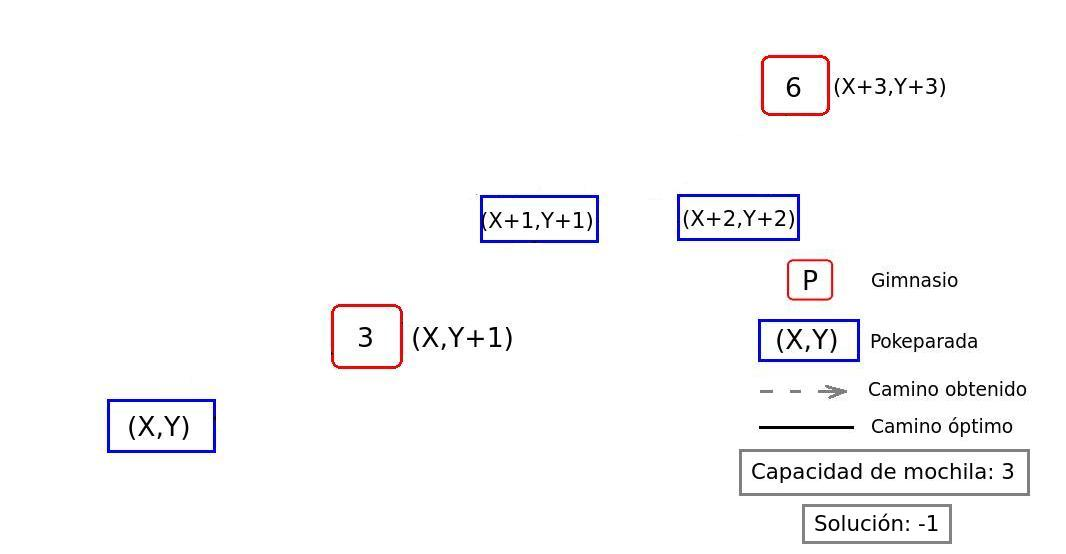
\includegraphics[scale=0.60]{./EJ2/sinSolucion.jpeg}
\\{\textit{Ejemplo 2.1 La soluci\'on obtenida es la \'optima: -1 (Sin soluci\'on)}}
  \end{center}
  \vspace*{0.3cm}
  
  \vspace*{0.3cm} \vspace*{0.3cm}
  \begin{center}
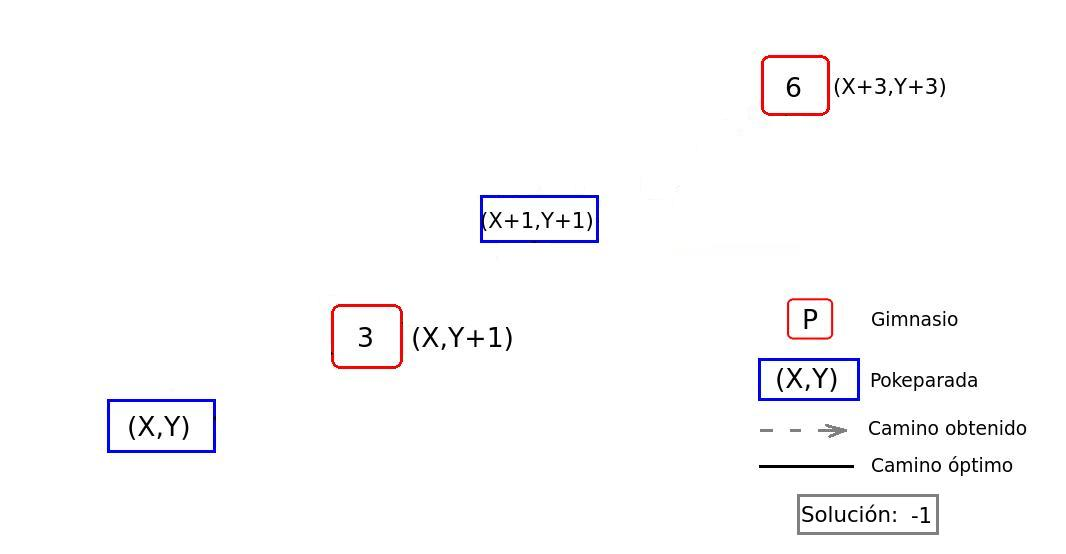
\includegraphics[scale=0.60]{./EJ2/sinSolucion1.jpeg}
\\{\textit{Ejemplo 2.2 La soluci\'on obtenida es la \'optima -1 (Sin soluci\'on)}}
  \end{center}
  \vspace*{0.3cm}


/---> FALTA LA MEDICION CON EL GRAFICO DE TIEMPOS

\begin{center}
\textbf{Familia 3}
\end{center}

En este caso, como nuestro greedy chequea si hay algun gimnasio a ser vencido con la cantidad de pociones que se tienen en el momento (se inicia con 0), y como todos necesitan 0, recorre los gimnasios sin necesidad de pasar por las pokeparadas, obteniendo la mejor soluci\'on posible.

  \vspace*{0.3cm} \vspace*{0.3cm}
  \begin{center}
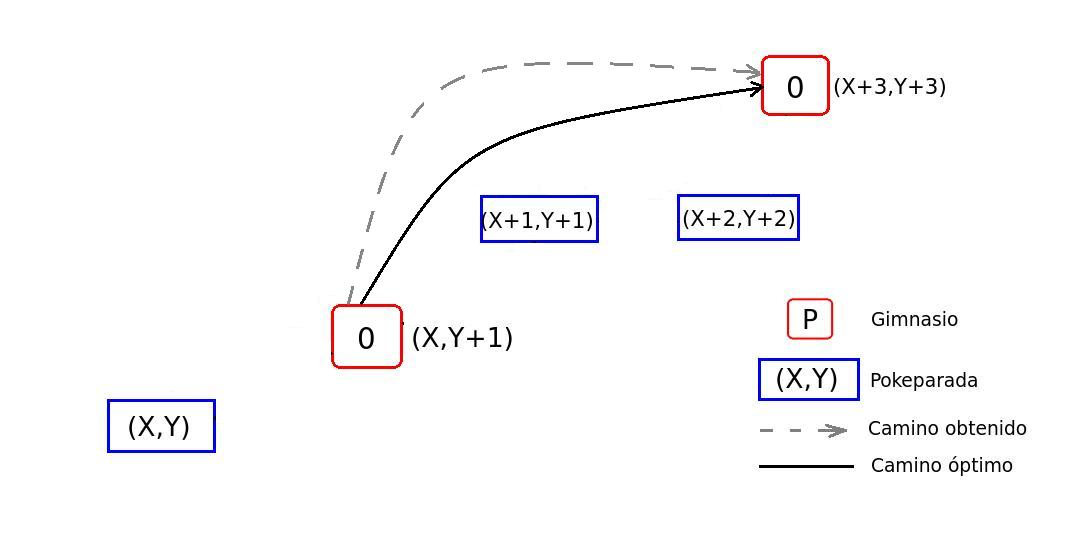
\includegraphics[scale=0.60]{./EJ2/gym0.jpeg}
\\{\textit{Ejemplo 2.3 La soluci\'on obtenida es la \'optima (Devuelve el camino optimo de recorrer todos los gyms)}}
  \end{center}
  \vspace*{0.3cm}


\begin{center}
\textbf{Familia 4}
\end{center}

Se obtendr\'a la soluci\'on \'optima ya que, se reciben primero pokeparadas para vencer a un gimnasio cerca de ellas y luego m\'as pokeparadas para vencer a otros gimnasios que se encuentren cerca de estas \'ultimas, se mostrar\'a a continuaci\'on un dibujo que ejemplifica lo dicho:

\vspace*{0.3cm} \vspace*{0.3cm}
  \begin{center}
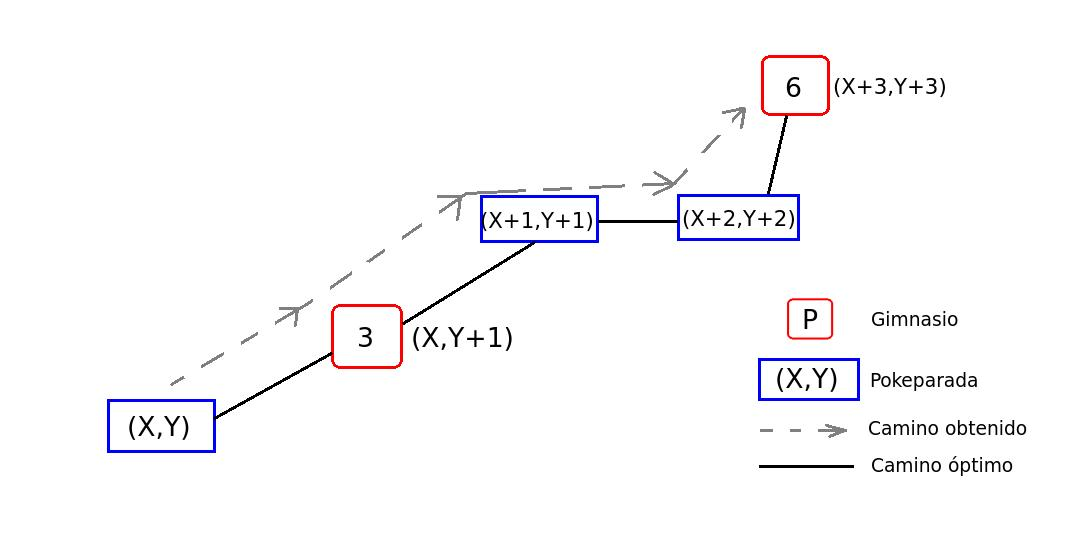
\includegraphics[scale=0.60]{./EJ2/optima.jpeg}
\\{\textit{Ejemplo 2.4 - La soluci\'on obtenida es la \'optima}}
  \end{center}
  \vspace*{0.3cm}

En cambio, no se obtendr\'a una soluci\'on \'optima cuando en vez de juntar una determinada cantidad de poder para vencer varios gimnasios consecutivos, el algoritmo decida ir a una pokeparada y luego a un gimnasio a derrotarlo, para luego repetir esta secuencia.

\vspace*{0.3cm} \vspace*{0.3cm}
  \begin{center}
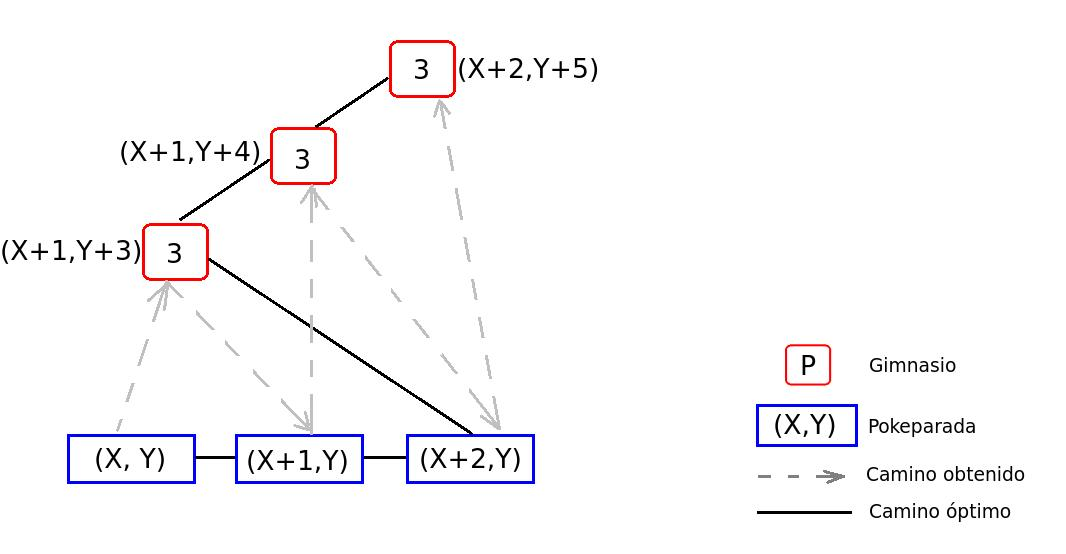
\includegraphics[scale=0.60]{./EJ2/nooptima.jpeg}
\\{\textit{Ejemplo 2.5 La soluci\'on obtenida no es la \'optima}}
  \end{center}
  \vspace*{0.3cm}
  
  
\vspace*{0.3cm} \vspace*{0.3cm}
  \begin{center}
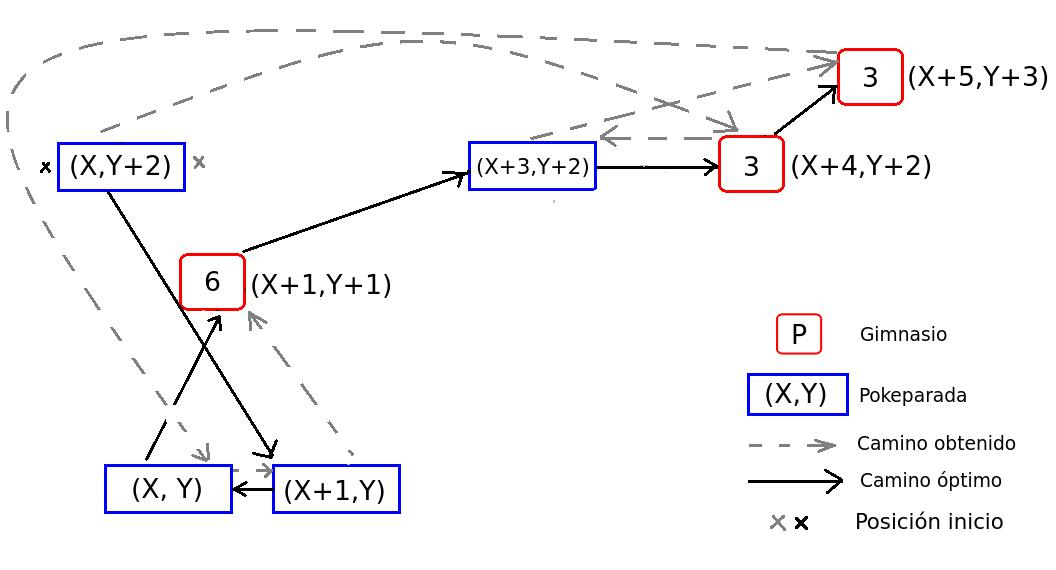
\includegraphics[scale=0.60]{./EJ2/nooptima2.jpeg}
\\{\textit{Ejemplo 2.6 La soluci\'on obtenida no es la \'optima}}
  \end{center}
  \vspace*{0.3cm}

La soluci\'on obtenida distará tanto de la óptima como la cantidad de veces que el algoritmo recorra una pokeparada y luego un gimnasio a vencerlo, sin importar si lo más optimo era pasar primero por las pokeparadas juntando poder y luego visitar varios gimnasios consecutivamente venciendolos a todos.
El peor caso será cuando el mapa sea un anillo de pokeparadas con un anillo interno o externo de gimnasios. 
El algoritmo iniciará en una pokeparada, luego irá a ganar a un gimansio con distancia mínima dentro de los gimansios no visitados, y siguiendo este recorrido, volverá a una pokeparada que se encuentre a una distancia menor de la pokeparada previa.\\

Se puede observar en el ejemplo 2.5 como nuestro algorimo va a la primer pokeparada y de ah\'i va a vencer al gimnasio m\'as cercano en vez de ir a la pokeparada que se encuentra inmediatamente consecutiva. Esto lo hace hasta vencer a todos los gimnasios.
Este estilo de caso será uno de los peores en referencia a la solucion obtenida que se obtenga ya que la misma ser\'a muy distante a la optima
